\begin{refsection}
    \renewcommand{\thefigure}{\arabic{figure}}

    \chapterTwoLines
    {Dispositivo moda}
    {a roupa em processos artísticos contemporâneos}
    \label{chap:dispositivo}
    
    \articleAuthor
    {Violeta Adelita Ribeiro Sutili}
    {Mestranda em Artes Visuais na Universidade Federal do Rio Grande do Sul (UFRGS)/ Minter Universidade Federal do Amazonas (UFAM), na área de concentração de Poéticas Visuais, na linha de Desdobramentos da Imagem. É pós-graduanda em Gestão Cultural (SENAC) Bacharela em Moda pela Universidade do Estado de Santa Catarina (UDESC, 2019). ID Lattes: 4199.3411.8974.7319. ORCID: 0000-0003-2333-5543. E-mail: violetasutili@gmail.com.}

    \begin{galoResumo}
        \marginpar{
            \begin{flushleft}
            \tiny \sffamily
            Como referenciar?\\\fullcite{SelfSutili2021}\mybibexclude{SelfSutili2021}, p. \pageref{chap:dispositivo}--\pageref{chap:dispositivoend}, \journalPubDate{}
            \end{flushleft}
        }
        A compreender a moda enquanto este grande sistema comunicador ocidental, formado por códigos distintos, o qual age de forma direta na construção de padrões estéticos e culturais, e que, de forma similar, cada época e localização geográfica impõe seu próprio arquétipo de beleza, pretende-se apontar manifestações artísticas que rompem com seu viés padronizador na vestimenta. A demonstrar obras brasileiras capazes de atravessar seus sentidos, por meio da atribuição do desenvolvimento de campos semânticos, são apresentada proposições artísticas brasileiras contaminadas pelo tema. Partindo da produção contemporânea de Nazareth Pacheco, artista em questão a apresentar um breve panorama acerca da representação de corpos e vivências através das vestes, posteriormente são apresentados trabalhos pessoais desenvolvidos em acordo, ou desacordo, aos processos de vestimentares.
    \end{galoResumo}
    \mednobreak
    \galoPalavrasChave{Corpo. Moda. Arte. Processos artísticos.}
    
    \begin{otherlanguage}{english}
    
    \fakeChapterTwoLines
    {Fashion device}
    {clothing in contemporary artistic processes}

    \begin{galoResumo}[Abstract]
        Undestanding fashion as this big Western communication system composed of different codes, which acts directly in the construction of aesthetic and cultural models and, the same way, each time and geographic location imposes a beauty archetype of its own; we aim to point out artistic manifestations that break with their standardizing bias on clothing. Demonstrating Brazilian works capable of surpass their own meanings, with the attribution development of semantic fields, Brazilian works that transcend common sense were exhibited and proposals for Brazilian art contaminated by the theme were presented. Beginning with contemporary works by Nazareth Pacheco, the artist briefly presented the process of representing the body and experience through vestment, and then introduced personal works that were developed in compliance with dressing processes, or not.
    \end{galoResumo}
    \mednobreak
    \galoPalavrasChave[Keywords]{Body. Fashion. Art. Artistic Processes.}
    \end{otherlanguage}

    \section{Introdução}

    Esta investigação apresenta-se como parte do processo de pesquisa interessada em compor diferentes colocações para as relações estabelecidas entre artes visuais e moda, bem como o fazer das roupas. Neste cenário, a roupa concomitantemente com processos artísticos de diferentes níveis práticos mostrou-se interessante objeto de interação entre indivíduos em suas aparições contemporâneas de acordo com seu momento histórico. 

    Neste texto, discutiremos os objetos da roupa como plataforma em processos artísticos, assim permeadas pelos corpos envolvidos na experiência de moda. Revertendo ao contrário do que seria a situação usual, as roupas nesta abordagem não são consideradas como simples objetos de consumo globalizado, mas como uma interface para as variadas aparições do corpo. Pensaremos as roupas como substância ou mesmo elementos mediadores em relacionamentos de exteriorização e processos de subjetivação. 

    Para vários fins, pode-se ter a roupa como uma espécie de envoltório, ou seja, a segunda pele que nos é aderida socialmente. Segundo \textcite[p.~34]{Mendonca2006Reflexo}, as principais necessidades ou finalidades das roupas podem ser atribuídas basicamente a três aspectos: proteção, humildade e decoração. Em várias etnias, em épocas diferentes, há uma ou mais finalidades para o uso de roupas e enfeites. 

    De forma ligeiramente inicial, é a partir do uso de adereços e da pintura corporal em pode-se percebê-los como itens utilitários para a experiência da vida: proteção, quando se busca nas roupas certo abrigo climático devido a temperatura local, ou o uso de roupas e artigos/amuletos de proteção espiritual. Seja por razões religiosas como estéticas, historicamente as vestes se apresentam como elemento visual para além de se cobrir o corpo. Nisto pensamos a roupa em si isolada de seu contemporâneo significado, este conhece-se por ser atrelado a complexas redes de troca e monetarização de serviços. 

    A roupa, mesmo que escalonada a sua presença capital, é um meio de expressão pessoal, um sinal de identidade e uma forma possível de estabelecer diálogos com o que há em seu entorno. Também podemos dizer que as vestes são o contato mais íntimo com o contexto exterior, de acordo com \textcite[p.~36]{CastilhoAndMartins2005Discursos} acredita-se que as relações entre roupa e corpo engendram ``as relações com mundos possíveis e imaginários, cujos significados são atrelados culturalmente à imagem e à percepção do ser''.

    Não obstante, pensar em roupas em circunstâncias atuais direciona a pesquisa a posicioná-las, meramente em um primeiro momento, a um sistema de primazia a novidade e ainda assim obsolescência de produtos, este ingenuamente é denominado moda: 

    \begin{quotation}
        Em sentido lato, a moda compreende todas as manifestações exteriores de usos e costumes consagradas dentro de um determinado período, desde comportamentos sociais e conceitos morais, até o estilo prevalecente nas formas dos objetos produzidos e do vestuário adotado. Em sentido restrito, o termo aplica-se às transformações periódicas nas formas dos trajes e demais detalhes de ornamentação pessoal. \cite[p.~17]{Mendonca2006Reflexo}.
    \end{quotation}

    Esse sistema cíclico composto por infindáveis expressões e ilusões de aparência ajuda a colocar as roupas em uma complexa rede de subjetivação simbólica. A roupa, em suas possibilidades, não é cabível de apresentar-se apenas como roupa, mas também pode vir a compor a arquitetura de uma afirmação social, intelectual e emocional de si mesmo e de seu coletivo, em que se coloca como elemento possível não apenas de cobrir o corpo, mas comunica-lo. Os trânsitos obtidos na troca de roupas demonstram discussões a nível oncológico, como quais são as preferencias em escolha, quais os lugares a ocupar no mundo. Golpeada por uma grande contradição, torna o indivíduo único, mas ao mesmo tempo pertence a um grupo.  

    Contudo, seria ingênuo emalhetar a dimensão estética e sensível das roupas às intempéries do que se compreende como o sistema de moda. Interessa-nos destacar que a moda cabe a gama expressiva vestimenta que se comporta na arquitetura têxtil do cobrir o corpo, a própria não se faz digna de tamanhos elogios quando este é dado teoricamente como o fenômeno social que possui aparição no início das atividades capitalistas na modernidade europeia, trazida e imposta aos povos de onde hoje encontra-se o território por nós habitado ao sul global.  

    \begin{quotation}
        A intervenção etnográfica nos estudos sobre moda problematiza este conceito e busca inserir os povos não ocidentais dentro de um sistema de produção do vestuário que antes era tido como apenas Ocidental. Em resumo, politiza-se o conceito de moda quando aplicado às análises históricas, culturais e sociais sobre a moda, localizando os efeitos sociopolíticos de uma abordagem que busca afirmar não haver moda em sociedades fora do Ocidentais. \cite[p.~16]{Santos2020Analise}.
    \end{quotation}

    Apresentada nossa inclinação teórica, interessa-nos, nas manifestações artísticas apresentadas, dialogar com diferentes abordagens da vestimenta, talvez rompendo com ultrapassadas impressões de moda, a tendo como campo vasto de expressão.

    \section{A roupa nos corpos e por que a moda?}

    Objeto responsável pela captação de diversas discussões, a moda tem em si relevante pesquisa realizada pelo filósofo francês Gilles Lipovetsky, a demonstrar que a mesma poderia ser dada como plataforma capaz de captar as subjetividades do corpo (e os seres que o possuem) através do vestir. ``Primeiro grande dispositivo a produzir social e regularmente a personalidade aparente, a moda estetizou e individualizou a vaidade humana, conseguiu fazer do superficial um instrumento de salvação, uma finalidade de existência'' \cite[p.~39]{Lipovetsky1989Imperio}.

    É neste campo de percepção que coloca-se o vestir, ocidentalmente performado através do fenômeno de moda, dentro do campo de processos de subjetivação. Ora, os sujeitos constituem sua vestimenta, e nisto sua aparência, através da construção por muitas vezes etérea de sua imagem e discurso e, uma vez que o sistema de moda se impõe no cotidiano de certas sociedades em seu viés colonizador, este é imposto e apropriado pelos indivíduos como canal de sua comunicação uma vez que o vestir constrói sua experiência cotidiana. A subjetividade na construção da vestimenta se faz presente, entretanto, seria ingênuo colocar que sua formação se dá de forma não estigmatizada em seus contornos por meio do viés colonizador que já lhe aplica a que compasso deveria surgir o contorno de seus corpos. 

    Como se é de costume, o vestuário pode determinar o nível de participação social vindo de seu usuário bem como discorre sobre sua inserção - a produção em massa de roupas vem a facilitar esse processo uma vez que o acesso a significativos bens se torna menos estratificado ao passo que a produção exponencial de roupas desvinculada de suas preocupações humanitárias ou trabalhistas lhes serve na redução de seus verdadeiros custos. Quase que na mesma metáfora de acesso a bens de vestuário contemporaneamente, a distinção pessoal também pode ser acessada, causando diferenciação entre os mesmos. Assim, por mais que uma peça de roupa seja adentrada em seu padrão industrial e reproduzida massificadamente esta mesma, ao ser posta em posse por determinado indivíduo, atribui a esta sua ferramenta de subjetivação: ao encontrar o corpo uma roupa não pode mais ser a mesma. 

    Os processos de subjetivação da vestimentar ocorrem ao passo que sua plataforma comunicadora é proposta ao universo pessoal de cada um, mesmo que se pense que o ato de criação não se ocorre em dado momento, a apessoalização (no sentido de tomar forma de quem a usa, humanizar) se mostra presente. Enquanto houverem exponenciais gamas de corpos e territórios corporais a serem vestido, a roupa não possuirá em si sua mesma aparência. Ora massificada, a roupa constituída em escala industrial, desprende-se de seu histórico inicialmente capitalista, e demonstra em si a auto representação de quem a veste. 

    Entretanto, se o desejo deste texto apresenta-se no debate das plataformas artísticas e expansões do corpo, por que moda? A compreender a moda enquanto este grande sistema comunicador ocidental, formado por códigos distintos, o qual age de forma direta na construção de padrões estéticos, e que, de forma similar, cada época e localização geográfica impõe seu próprio arquétipo de beleza, pretende-se apontar manifestações artísticas que rompem com seu viés padronizador na vestimenta (e em seu teor conceitual, talvez, rompam com a ``moda''). Mesmo considerando a moda como este ser estigmatizado de corpos com sua fundação no início da atividade capitalista na modernidade europeia, ainda que se possível removê-la em nossa globalização de seu perfil neocolonialista, se coloca presente os processos subjetivos (conscientes ou não) de seus usos. A moda não se mostra aqui como campo do consumo e fetiche, mas também como linguagem apropriada por meios artísticos em sua dimensão vestimentar. 

    Nesta discussão, não se poderia citar as vestes apenas como ``roupas'' utilizadas por artistas em suas manifestações, afinal, a percepção do mesmo quanto ao uso delas é deturpada pela construção da lógica vestimentar em que vive. A aparência de como conhecemos uma calça, por exemplo, é calcada na apresentação da mesma que nos foi imposta a partir do projeto colonialista, assim se dá com camisas, casacos, etc.: as roupas que conhecemos não são necessariamente as roupas que nossa lógica histórica veio a criar.  

    A ideia de moda vinculada a plataformas artísticas nos casos apresentados se faz presente com aparições do vestir que não dialogam com trajes tidos como pertencentes a moda ou indumentária. Tal termo considerado de cunho colonialista ou necolonialista uma vez que se impõe em situações de diálogo binário: a moda relacionada ao novo e a mudança, e as sociedades não ocidentais presas ao seu tempo. 

    \begin{quotation}
        Entendemos que o conceito de moda pode ser utilizado como mais uma noção dentro do aparato ideológico colonial que busca desautorizar a relação das sociedades não ocidentais com o tempo ao afirmar que esta última não tem moda porque pouco mudam seu vestuário, ou como o colonizador prefere chamar, sua indumentária ou costume \cite[p.~6]{Santos2020Analise}.
    \end{quotation}

    É neste limiar que se discute quando ocorrem manifestações artísticas capazes de romper com as convenções ordinárias das vestes e que são. Captadas transbordando suas fronteiras utilitárias (proteção física e temperatura) e excedendo a vasta expressão subjetiva de cada ser que se apresenta vestindo e traduzindo a seus modos sua recém adquirida peça do sistema comercial de moda, as protuberâncias artísticas em roupas ocorrem quando se desvincula o universo de sua aparência ao preciso discurso pessoal. Emendar as vestes ao discurso artístico pessoal também revela subjetivações provindas das manifestações por meio dos signos destas vestes, produzindo novas variações para seus significados.  

    Dada a perspectiva da produção de subjetividade engendrada pelo uso apropriado de peças do vestuário, seja em sua prática cotidiana ou a nível do objeto na arte, a moda é tomada como dispositivo. Este desdobramento de conceito é demonstrado pelo filósofo francês Michel \textcite{Foucault1979Microfisica} e também articulado nos estudos dos filósofos Gilles \textcite{Deleuze1990Que}. A escapar das diferenças de suas abordagens, a ideia de um dispositivo pode ser compreendida como uma rede heterogênea em que nestas se engendram práticas disciplinares e de controle. Destas mesmas, se articulam discursos, regras, instituições. O tramar de suas ações produzem modos de pensar, formas de viver, sentir e suas visualidades.  

    Uma das ferramentas que se mostram ativas no dispositivo de moda são suas próprias modelagens, desenho planificado de cada pedaço de tecido necessário para a construção e uma roupa. Tais modelagens, juntamente de seus limites, agregam uma lógica normativa de corpos e expressões, ao desenhar o contorno do corpo também se impõe a forma do mesmo. Entre outros problemas, esses limites postos pela moda dentro da dimensão do vestir também estimulam o não alargamento de discursos e representações. 

    Contudo, apesar de dadas relações não favoráveis a multiplicidade comunicacional, o elemento vestível, por estar sempre extremamente próximo de seus usuários, ainda assim é demonstrado presente em seus desdobramentos como plataforma criativa. Deste modo, emergem manifestações contrárias à sua homogeneidade, trabalhando na transpessoalidade daquilo que lhe é condicionado. Tamanha sua abordagem conceitual, as manifestações artísticas que em si buscam o romper com o viés padronizador das roupas utilizam-na do avesso, colocando em jogo o modo de funcionamento do próprio dispositivo. 

    Assim, partindo dos processos de subjetivação engendrados ao vestir e o uso das roupas delineadas pelos corpos presentes, se demonstra apropriado o estudo desta plataforma na arte. As escolhas artísticas, quando em decorrência do viés vestimentar explora suas possibilidades, seus diálogos, sua abrangência, de forma a compreender a potencialidade de seus discursos quando apropriados de materiais cotidianos. Quando o discurso se apresenta, em sua esfera participativa, aos interesses em diálogo com possíveis receptores, contribui-se para a evasão de ideias e pensamentos permeados em suas narrativas por seus territórios e culturas. 

    De acordo com \textcite[p.~75]{Costa2009Roupa},

    \begin{quotation}
        [\dots] o traje, por envolver identidade, sexualidade, poder e sentidos metafóricos, constitui um meio fascinante, além de tocar em aspectos como intimidade com o corpo e expressão de status, significados simbólicos e de comunicação.
    \end{quotation}

    Costa coloca assim, o traje como ``objeto de reflexão, meio de expressão e suporte de criação'', podendo oferecer a este que o faz uso, no caso, o artista ``espaço e substância para a obra de arte''. O traje, por estar presente ao corpo, comunica sua identidade, sexualidade, entre outros, construindo seu campo sensível pertinente ao olhar de quem o veste e aquele que o recebe. Proposto por Cacilda Teixeira da Costa \citeyear{Costa2009Roupa}, aplica-se o termo ``roupa de artista'' o qual abrange todo o tipo de obras que demonstrem roupas não sendo necessariamente destinadas a uso.

    O termo ``Roupa de Artista'':

    \begin{quotation}
        [\dots] designa uma produção que se insere no campo dos novos meios, ao lado do vídeo, arte postal, cinema de artista, web art e outros, já esteve presente em quase todos os movimentos artísticos do século XX, na forma de vestimentas singulares, performances, empacotamentos, estamparias exclusivas, vídeo e outras tecnologias e continua contemporaneamente em transposições, apropriações e vestuários incomuns, entre outras manifestações. \cite[p.~9]{Costa2009Roupa}.
    \end{quotation}

    Em sua proposta, interessa-nos estuda-la a partir dos usos da roupa na arte em suas manifestações destoantes ao povoado sistema de moda, entendido metaforicamente como esta catraca apaziguadora de expressões distintas a complexidade neocolonial imposta. Uma vez apresentada para manifestar a presença daquele que a veste, dirige-se a experiência vivida, a narrativa encontrada ao perceber a roupa como portadora de um ser vivente. Moda e roupas apresentam-se como seres interdependentes neste cenário, mas não incapazes de fazer ressoar importantes questionamentos em seu campo ampliado. 

    As roupas atribuem um novo significado na arte. Tida como plataforma cotidiana de uso comum, o explorar das vestes demonstram captações de imaginários e representações dadas pela narrativa individual de quem as atribui a sua aparência, discurso, ou caminhada artística. Por meio de uma breve análise das pesquisas sobre os artistas e suas obras no vestuário aqui apresentadas, podemos perceber que muitos deles passam a pensar no ato de vestir a partir de novos preceitos e povoações, como os sentidos despertados, a crítica a padronização de corpos e outras questões que envolvem a narrativa daqueles que possuem seu contorno. 

    \section{O vestir de Nazareth Pacheco}

    A artista Nazareth Pacheco, natural de São Paulo, apresenta sua carreira que começou em meados da década de 1980. A partir do início da década de 1990, passou a usar materiais cortantes agregados aos seus trabalhos, produzindo em suas obras determinadas experiências. Criava então objetos ou obras por muitas vezes ``intocáveis'', não acessíveis a mão com tanta facilidade. Encontramos o contraste entre o que será a sedução e a repulsa na biblioteca de imagens derivadas de sua experiência biográfica, seus registros tomam presença em sua aparição, essas impressões envolvem conceitos universais a vivencia humana como dor, prazer, morte e vida.  

    Autora de trabalhos como roupas inteiramente feitas de navalha, a artista estuda as questões de memória e identidade de dentro para fora. Desde sua infância, a artista passou por diversas operações cirúrgicas devido a doenças congênitas, que se caracterizam por uma relação dolorosa com o corpo e as lâminas que a atravessavam com certa frequência.	 

    Embora suas obras citem diretamente essa experiência, seus trabalhos não podem ser classificados apenas como suas práticas autobiográficas, pois neles expõe a universalidade do sofrimento, sendo este também uma característica da vida e das condições de sobrevivência neste mundo o qual se habita. Os trabalhos de Nazareth Pacheco se equilibram e testam, diante a análise de quem vos escreve, a dicotomia entre charme e estranheza: vistos à distância, são objetos ou peças delicadas e brilhantes, atraem o olhar com vislumbre. Se mostram materiais como miçangas e cacos de vidro ou resina acrílica, a curta distância se proclama: materiais cortantes e perfurantes como facas, ganchos e navalhas, causam sentimentos de angústia e até medo \cite{Pereira2012Memorias}.

    Em busca de uma explicação ampliada, a partir do olhar as peças feitas pela artista (roupas e acessórios específicos para corpos femininos) podemos envolver a dimensão violenta das cirurgias estéticas, que transforma o corpo feminino em busca de se adequar aos padrões de certa ``normalidade''. A adaptabilidade presente, ou seja, se pensarmos em \textit{corsets} ou outros tipos de traçados projetados para corpos-modelo, em que buscamos a aceitação social e a tolerância do vestuário e da própria moda, para que as vestes tenham as mesmas dimensões violentas no corpo. Um modelo ao caminho da forma corporal ideal ou perfeita. Até mesmo, aplica-se a esta discussão, as formas do corpo reproduzidas a nível industrial pela cadeia de atividades manufatureiras de produção do vestuário: desenha-se um formato de corpo e espera-se que um grande escopo populacional se insira no mesmo. 

    O fato de permitir que o corpo suporte tais ataques de forte característica invasiva, o faz perder a dimensão do significado da persuasão colocada ao corpo que se entende como incorreto e ineficaz no enfrentamento desta situação. Uma vez que se apresente padronizado, brilhante, charmoso e sedutor, isso faz com que valha a pena o processo intrusivo e violento de modificação da aparência. A artista relata assim que quando se busca uma sensação de beleza, se faz necessário sucumbir a cortes, não necessariamente estes propostos em cirurgias plásticas, mas também a evasão de nossos corpos quando desiste-se deles como são e o subordinam a compreensão de imagem corporal desejada coletivamente. Assim expõe sua relação biográfica pessoal no processo de trabalho, e o ideal de beleza passou a ser a prioridade. Para a artista, o bisturi a traz o pânico, entretanto, esse é o caminho apresentado que precisamos percorrer para alcançar a chamada beleza. 

    Apresentada na Figura \ref{fig:vestido-acrilico}, o vestido composto de lâminas de barbear, compõe um simulacro de brilho e leveza atribuída em sua transparência e caimento, como uma cortina de missangas, as quais, em um olhar mais atento, denunciam um objeto perigoso.

    \begin{figure}[ht]%
        \centering%
        \caption{``Vestido Acrílico, Cristal e Giletes'', Nazareth Pacheco, 2003}%
        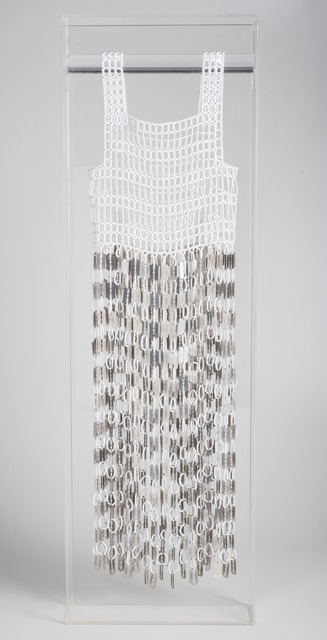
\includegraphics[width=.5\textwidth]{articles/13-dispositivo-moda-a-r/image1.jpg}%
        \caption*{Fonte: Editora PUC-RS. Disponível em \url{http://ebooks.pucrs.br/edipucrs/anais/apcg/edicao10/Hiascara.Alves.pdf}. Autor: Hiascara Alves.}%
        \label{fig:vestido-acrilico}%
    \end{figure}%

    A imagem apresentada na Figura \ref{fig:vestido-acrilico} mostra o trabalho de Nazareth Pacheco, nele a artista propõe o vestido de giletes assim feito rigorosamente sob suas próprias medidas. Este representa sua presença em objeto, por outro ângulo quando o observamos desprovido de um corpo, automaticamente nos colocamos em seu lugar. A medida que passamos a habitá-lo, a experiência ocorre estabelecendo uma relação empática que nos desloca do lugar comum, que subverte e transforma os modos de vestir, que nos fazem refletir sobre as manifestações da existência em nossa sociedade e de como um objeto aparentemente trivial como uma vestimenta é imbuído de uma significação que transborda à nossa vista.

    Sob o ponto de vista da leitura que é realizada acerca de seus trabalhos, é nesse movimento em zig-zag, em que reconstrói e reforça conceitos, estereótipos e tradições. O receptor diante da obra sente a tecitura cortante do vestido de Pacheco que dilacera a própria pele, expondo a dimensão sensorial de seu sangue e carne. É vivida a fragilidade e vulnerabilidade da vida, não apenas, apresenta-se o enredo do ``ser mulher'' para algumas, que diante de sua infinidade de papéis de gênero percorrem o caminho de encontro ao belo ao qual se sentem no dever de servir.

    \begin{figure}[ht]%
        \centering%
        \caption{Detalhe lâminas utilizadas}%
        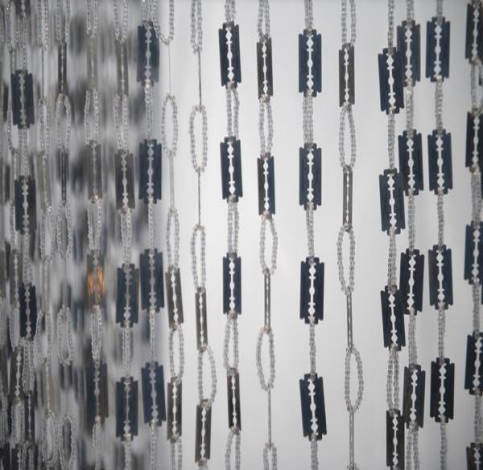
\includegraphics[width=.75\textwidth]{articles/13-dispositivo-moda-a-r/image2.jpg}%
        \caption*{Fonte: Editora PUC-RS. Disponível em \url{http://ebooks.pucrs.br/edipucrs/anais/apcg/edicao10/Hiascara.Alves.pdf}. Autor: Hiascara Alves.}%
        \label{fig:detalhe-vestido-acrilico}%
    \end{figure}%

    \section{Processos pessoais}

    Vista a dissidência em foco a aparições em moda, uma nova dimensão é proposta para as vestes, os objetos nas roupas vêm a se fundir, não se trata exclusivamente do objeto roupa como a aparição de seus signos ao compor artístico. Estes contágios ocorrem de forma perene, bem como as práticas no espaço que passa a ser a superfície, seja este corpo, tecido, roupa. O habitar em todas suas dimensões se torna pele, a roupa mostra se como este tecido sensível e, até mesmo em sua ausência, onde ocorrem estas habitações é proposta a escrita. Ao adentrar na dimensão do vestível, veste-se, de modo que vestir o próprio objeto é colocá-lo a discurso de si. 

    Neste cenário, diferentemente da terminologia aplicada as roupas, o termo moda denomina, nesta concepção, o modo de pensar e viver estabelecido na modernidade europeia, e nos primórdios da atividade econômica capitalista, a qual prima pelo novo e abandona-se a tradição. A compreensão conceitual de moda é capaz de tomar amplas variações de acordo com a autoria de quem a investiga, o que se busca discutir aqui é o processo da aparência ao sistema de moda em colisão ao que se compreende como a roupa: canal de comunicação-codificação de subjetividades-espaço em trânsito. Ou o inverso. 

    Os seguintes trabalhos apresentados se introduzem como processos em tramar a tessitura das vestes. Utilizou-se de abordagens que pensassem a arquitetura técnica da moda, atribuindo aos trabalhos objetos presentes no cotidiano fabril de moda, como fichas técnicas, desenhos técnicos, nomenclaturas próprias e ordens de execução. Criava-se então objetos ou obras por muitas vezes ``segmentadores'', objetos aos quais facilmente seriam utilizados para categorizar elementos, pessoas, corpos. É encontrado o contraste entre o que será a padronização e o não cumprimento as exigências técnicas estabelecidas na experiência de submeter-se ao vestir moda, seus registros tomam presença através da aparição de linhas, caixas. Esses limites envolvem conceitos cotidianos no que se diz respeito a vestes, movimentos, tamanhos e expressões. 

    Ao apresentar trabalhos compostos exclusivamente das visualidades de linhas e limites, estuda-se as questões de sobreposição de fronteiras e padronizações corpóreas na imagem de moda imposta. Assim como os limites do corpo são traçados e impostos no desenvolvimento de peças de vestuário, impõe-se o contorno desejado e os modos de viver por assim desejados. Apesar destes limites, a camada expressiva vestimentar se coloca proposta a cruzar padrões e hábitos. 

    De tecido praticamente transparente e linhas de tensão em seu entorno é construído uma espécie de \textit{body}, peça de roupa voltada a parecer com o contorno do corpo nu. Por meio de costuras bruscas desenha o contorno de cada molde da peça, cada engrenagem de limitação de seu dispositivo. A modelagem da roupa, desenha um corpo magro e esguio, em seus doze moldes, reúne diferentes recortes de tecido que modelam um corpo ausente, mas ainda tensionado por seus contornos, cabe a peça buscas aquela que a vista e cumpra com suas limitações, ainda que exposta. Após o amadurecimento de sua identidade, a roupa recebe a própria ficha técnica, ``a qual contém todas as informações técnicas necessárias do produto a ser desenvolvido'' \cite{Pires2014Ficha}. Nela apresenta suas bruscas atribuições, registros de tensão e pressão, em toda sua anatomia. São nomeados os moldes, e mais grosseiramente: é apresentado seu processo.

    \begin{figure}[ht]%
        \centering%
        \caption{Ficha técnica}%
        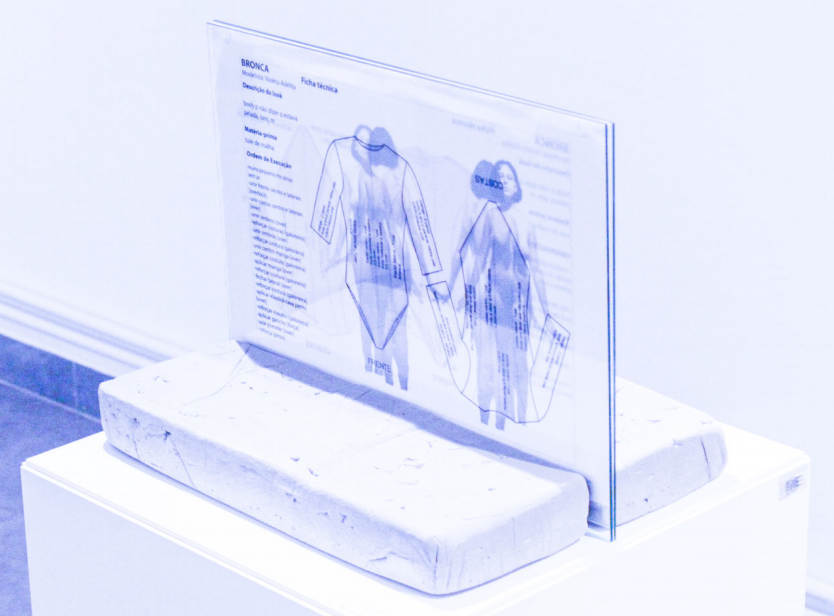
\includegraphics[width=.75\textwidth]{articles/13-dispositivo-moda-a-r/image3.jpg}%
        \caption*{Autor: Violeta Sutili.}%
        \label{fig:ficha-tecnica}%
    \end{figure}%

    Assim, veste-se do \textit{body} e sua ficha técnica, onde demonstra-se registro de nova habitação. Esta peça possui sua vida social arraigada nas demonstrações que é colocada, vindo de encontro a proposta inicial que possuía: somos desenhados e imbuídos em numeradas situações. Por sua vez, estes contornos mesclam-se com a roupa, o corpo percorrido já é visto no seu simulacro vestido. 

    Esta materialização é realizada em papel vegetal, vidro e cimento. Em que a vivência cotidiana vestimentar encontra-se dentro do sanduiche de vidro, nas entranhas da ficha técnica, não como a força motriz do produto (como é a roupa) mas o dispositivo de constante ordem (como é a moda). 

    A visualidade e conceitualidade dos trabalhos apresentados (incluso o de Nazareth Pacheco) nada se apresentam na conceituação de moda e seu fazer ou, até mesmo, em seu processo de criação. Assim como o requinte e o comportamento são relegados às vestes, pelo contrário, há uma completa intenção de subverter o uso e representação de roupas (principalmente femininas), condenando explicitamente esta denúncia às condições físicas e imagéticas dos corpos em diferentes áreas que sistematizam o cotidiano social das aparências, desde o que lhe confere a gênero, como também espaços públicos, íntimos e inconscientes pessoais.  

    Estas e outras produções de sentido (e de participação feminina) dessas e de outras artistas em face das técnicas tradicionais, e das participações em acordo as expressões vigentes, demonstra que a linguagem dada pelos têxteis é ``uma cacofonia de muitas vozes que, como os tipos de obras feitas por artistas contemporâneos provam, não mostram sinais de esgotamento ou obsolescência.'' \cite{Bell2015New}. O que se mostra aqui é apenas um excerto, tentando revelar os muitos aspectos da experiência em vestes, a demonstrar o poder político dos trabalhos e a relevância de sua atuação como agentes dissidentes.

    \section{Considerações finais}

    Em diálogo com o cotidiano, as práticas artísticas contemporâneas levantam questões que enfatizam a relação entre arte e vida, podendo questionar o estilo de vida hegemônico vigente. Ao utilizar materiais incomuns (como roupas) como uma das formas de manipular essas provocações define-se a conversa não exclusiva ao debate dos corpos em jogo. Nesse caso, os vestidos de Nazareth Pacheco, bem como os corpos em Ficha Técnica, tornam-se uma plataforma que pode questionar os dispositivos de moda por contrastar os padrões gerados. 

    Os trabalhos apresentados demonstram ter seguido um caminho diferente dos requisitos de dispositivo. Ao usar uma variabilidade material inesperada, a construção do belo e a padronização dos corpos são questionados. Quando olhamos para as obras, não só o mercado, mas também os dispositivos de produção dos próprios equipamentos de moda são questionados em certa medida. Fazer suas próprias representações quanto ao pensar a produção de roupas, em vez de usa-la simplificadamente prontas como vendidas em grande escala, pode ser uma forma de resistir.  

    Mesmo ao reconhecer o sistema de moda como este ambiente hegemônico, a plataforma roupa propõe-se como substancia para a escritura de narrativas, imaginários e representações. Assim, ao aclamar suas historiais pessoais, os indivíduos que a utilizam expressivamente não apenas comunicam a si, mas comunicam sobre seu coletivo e suas crenças. 

    \begin{quotation}
        ``Como é que sabemos isso? Pelo próprio tecido.'' Isso acontecia não só porque a tecelagem, tal como a escrita e outras artes visuais, fosse frequentemente ``usada para marcar ou anunciar informação'' e como ``meio mnemônico para registrar fatos e outros dados'', mas também porque têxteis comunicam, de fato, em termos das imagens que aparecem no lado direito do pano, embora este seja apenas o sentido mais superficial em que processam e armazenam dados. \cite[p.~29]{Rago2013Aventura}.
    \end{quotation}

    Por fim, pode-se considerar que os processos artísticos apresentados demonstram-se como articulações dissidentes ao efeito hegemônico produzido pela linha de dispositivos de moda. Eles contradizem os principais padrões de vestimenta, a homogeneização e a lógica corporal imposta nesse dispositivo, assim, o desafiam ao propor outros métodos de manuseio do vestuário, que podem apresentar diferentes visões na produção subjetiva. 

    Se tivermos a roupa como este território que cobre o corpo, nada mais apropriado, em nosso contexto em que o mercado global mostra força ao definir as formas que se darão o vestir, que discutamos estas questões através da moda por si mesma. Deste modo, seria através de seus próprios moldes e incongruências humanitárias, zarpando de um corpo envolto que opera  

    \begin{quotation}
        [\dots] como suporte material, sensível, que se articula com diferentes códigos de linguagem, como a gestualidade, com a sensorialidade e com a própria decoração corpórea, e a moda e o seu design como projeto, processo de transformação da aparência que objetiva a diferenciação ou a similitude. \cite[p.~31]{CastilhoAndMartins2005Discursos}.
    \end{quotation}

    Mesmo em discordância com determinadas praticas em moda e seus impactos, a pesquisa alinha-se a pensar novas conceituações para a mesma, uma vez que não deixará de envolver os corpos, mas sim se demonstra necessário politizar seus conceitos. A fim de demonstrar narrativas de variados contextos, especialmente ao sul onde nos localizamos, parte-se de uma ideia de moda como plataforma e potência: do corpo e de seu indivíduo-coletivo.

    \begin{quotation}
        Pois bem, entendemos que a moda é uma forma de se relacionar com o vestuário, dentre muitas outras, devendo ser estudada como o que de fato ela é: uma das maneiras de se lidar com o vestuário não sendo melhor ou mais surpreendente que qualquer outra [\dots] neste sentido, o vestuário incorpora a moda, uma vez que esta última existe apenas como uma relação social que se estabelece com o primeiro. \cite[p.~21]{Santos2020Analise}.
    \end{quotation}

    \printbibliography[heading=subbibliography,notcategory=fullcited]

    \hfill Recebido em 3 mai. 2021.

    \hfill Aprovado em 4 mai. 2021.

    \label{chap:dispositivoend}

\end{refsection}
